\documentclass[12pt,a4]{article} %[font size, tamano de hoja]{Tipo de documento}

\usepackage[left=1.8cm,right=1.8cm,top=32mm,columnsep=20pt]{geometry}

\usepackage[utf8]{inputenc} %Formato de codificación
\usepackage[spanish, es-tabla, es-nodecimaldot]{babel}
\usepackage{amsmath} %paquete para escribir ecuaciones matemáticas
\usepackage{amssymb} %paquete para símbolos adicionales
\usepackage{float} %Para posicionar figuras
\usepackage{graphicx} %Para poder poner figuras
\usepackage{hyperref} %Permite usar hipervínculos 
\usepackage{multicol} %Para hacer doble columna
\usepackage{subcaption}
\usepackage{float}
\usepackage[sorting=none]{biblatex} %Imports biblatex package. To cite use \cite{reference_label}
\addbibresource{tp3.bib} %Import the bibliography file



\title{Análisis de Reducción de Dimensionalidad y Compresión de Imágenes utilizando Descomposición de Valores Singulares\\


\vspace{20mm}

 Métodos Numéricos y Optimización\\
 Trabajo práctico N$^{\circ}$3\\
}

\author{Timoteo Menceyra y Alejo Zimmermann\\ [2mm] %\\ para nueva línea
\small Universidad de San Andrés, Buenos Aires, Argentina}
\date{1er Semestre 2024}
% Tamanos de letra: 
% \tiny	
% \scriptsize
% \footnotesize
% \small	
% \normalsize	
% \large	
% \Large	
% \LARGE	
% \huge	
% \Huge


%Todo lo que está antes de begin{document} es el preámbulo
\begin{document}
\vspace{1cm} % Ajusta la distancia vertical entre la fecha y la imagen



\maketitle
% \begin{center}
% \includegraphics[width=5cm]{logoUdesa.png} % Ajusta la ruta y el tamaño de la imagen
% \end{center}


\begin{abstract}
Este informe explora la aplicación de la Descomposición de Valores Singulares (SVD) para la reducción de dimensionalidad y compresión de imágenes. Se analizan dos casos: reducción de dimensionalidad de un conjunto de datos multidimensional y compresión de imágenes. En el primer caso, se evalúa el impacto de diferentes dimensiones reducidas en la preservación de similitud entre muestras y el rendimiento de predicción lineal. En el segundo, se estudia la calidad de reconstrucción de imágenes comprimidas y la similitud entre imágenes en espacios de baja dimensión. Los resultados resaltan la eficacia de SVD como técnica para reducción de dimensionalidad y compresión de datos.\\
\vspace{2mm}
\end{abstract}


\raggedcolumns

\section{Introducción}
La Descomposición de Valores Singulares (SVD) \cite{burdenfaires} es una técnica fundamental en el análisis de datos y procesamiento de señales. Esta descomposición matricial permite factorizar una matriz en tres componentes: matrices ortogonales y una matriz diagonal de valores singulares. La SVD tiene numerosas aplicaciones, incluyendo la reducción de dimensionalidad y la compresión de datos.
La reducción de dimensionalidad \cite{linaer_algebra} es un proceso crucial en el análisis de conjuntos de datos de alta dimensión. Estos conjuntos a menudo contienen redundancias y ruido, lo que dificulta su visualización e interpretación. La SVD permite proyectar los datos a un espacio de dimensión reducida, preservando la mayor cantidad posible de información relevante y facilitando el análisis y la visualización de patrones subyacentes.
Por otro lado, la compresión de imágenes es una tarea fundamental en el procesamiento de imágenes digitales. Las imágenes digitales suelen requerir una gran cantidad de espacio de almacenamiento y ancho de banda para su transmisión. La SVD ofrece una técnica eficiente para comprimir imágenes, reduciendo su tamaño sin comprometer significativamente la calidad visual.
En este informe, se exploran dos casos de estudio que aprovechan la potencia de la SVD. El primero se centra en la reducción de dimensionalidad de un conjunto de datos multidimensional, analizando el impacto de diferentes dimensiones reducidas en la preservación de similitud entre muestras y el rendimiento de predicción lineal utilizando mínimos cuadrados. El segundo caso aborda la compresión de imágenes, estudiando la calidad de reconstrucción de imágenes comprimidas, la similitud entre imágenes en espacios de baja dimensión y determinando el número mínimo de dimensiones necesarias para garantizar un error de reconstrucción aceptable.




\section{Métodos}
En este trabajo utilizamos la Descomposición de Valores Singulares (SVD) para reducir la dimensionalidad de un conjunto de datos multidimensional y comprimir imágenes. 

\subsection{Descomposición de Valores Singulares (SVD)}
\label{SVD}
La Descomposición de Valores Singulares (SVD) es una técnica matemática que factoriza una matriz en tres componentes: una matriz de vectores singulares izquierdos, una matriz diagonal de valores singulares y una matriz de vectores singulares derechos. La SVD se define para cualquier matriz \(A\) de tamaño \(m \times n\) como:


\begin{equation}
    A = U \Sigma V^T= \begin{bmatrix}
    U_{1,1} & U_{1,2} & \cdots & U_{1,m} \\
    U_{2,1} & U_{2,2} & \cdots & \vdots \\
    \vdots & \vdots & \cdots & \vdots \\
    U_{m,1} & \cdots & \cdots & U_{m,m}
    \end{bmatrix}\begin{bmatrix}
    \sigma_1 & 0  &\cdots &0\\
    0 & \sigma_2  &\cdots &0\\\
    0 & 0 &\cdots &\sigma_ n\\
    \vdots & \vdots &\cdots &\vdots\\
    0&0&\cdots &0
    \end{bmatrix}\begin{bmatrix}
    V^{T}_{1,1} & \cdots \\
    \cdots & V^{T}_{n,n}
    \end{bmatrix}
    \label{svd}
\end{equation}




donde \(U\) es la matriz de vectores singulares izquierdos de tamaño \(m \times m\), \(\Sigma\) es la matriz diagonal de valores singulares de tamaño \(m \times n\) y \(V^T\) es la matriz de vectores singulares derechos de tamaño \(n \times n\).

\subsection{Reducción de dimensionalidad: Análisis de Componentes Principales (PCA)}
\label{PCA}
En la reducción de dimensionalidad, utilizamos el método de Análisis de Componentes Principales (PCA). PCA es una técnica estadística que permite transformar un conjunto de variables correlacionadas en un nuevo conjunto de variables no correlacionadas llamadas componentes principales. Estos componentes principales capturan la mayor parte de la variabilidad de los datos originales y se ordenan en función de su importancia.

El cálculo de PCA se realiza a través de los siguientes pasos:

1. Calculamos la matriz de covarianza de los datos originales.
2. Calculamos los autovectores y autovalores de la matriz de covarianza.
3. Ordenamos los autovectores en función de sus autovalores, de mayor a menor.
4. Seleccionamos los primeros k autovectores correspondientes a los k componentes principales.
5. Proyectamos los datos originales en el espacio de los k componentes principales.

La fórmula para la proyección de los datos originales en el espacio de los k componentes principales es:

\[
X_{\text{proy}} = X \cdot V_k
\]

donde \(X_{\text{proy}}\) es la matriz de datos proyectada, \(X\) es la matriz de datos originales y \(V_k\) es la matriz de autovectores correspondientes a los k componentes principales.



\subsection{Fórmula de similitud}
\label{similitud}
La similitud entre un par de muestras $x_i$, $x_j$ se puede medir utilizando una función no lineal de su distancia Euclidiana:
\begin{equation}
    K (x_i, x_j) = \exp \left( -\frac{|x_i - x_j|_2^2}{2\sigma^2} \right),
    \label{eq: Similitud}
\end{equation}


para algún valor de $\sigma$. Aquí, $|x_i - x_j|_2$ representa la norma Euclidiana o distancia Euclidiana entre los vectores $x_i$ y $x_j$. Esta función transforma la distancia Euclidiana en una medida de similitud, donde valores más cercanos a 1 indican una mayor similitud entre las muestras, y valores cercanos a 0 indican una menor similitud

\subsection{Cuadrados mínimos}
\label{cuads_mins}

Utilizamos el método de Cuadrados Mínimos utilizando la Descomposición de Valores Singulares (SVD) para resolver un sistema de ecuaciones lineales sobredeterminado, es decir, cuando el número de ecuaciones es mayor que el número de incógnitas.

Considere el sistema de ecuaciones lineales representado por $Ax = b$, donde $A$ es una matriz $m \times n$, $x$ es el vector de incógnitas de dimensión $n \times 1$, y $b$ es el vector de términos independientes de dimensión $m \times 1$.

Si $A$ es una matriz de rango completo, podemos aplicar la Descomposición de Valores Singulares:

\[
A = USV^t
\]

donde $U$ es una matriz $m \times m$ ortonormal, $S$ es una matriz diagonal $m \times n$ que contiene los valores singulares de $A$, y $V^t$ es la traspuesta de una matriz $n \times n$ ortonormal.

Como $A$ no tiene inversa para resolver directamente $Ax = b$, calculamos la pseudo-inversa $A^+$ y la aproximación de la solución $\tilde{x}$:

\[
A\tilde{x} = b
\]
\[
US V^t \tilde{x} = b
\]

Multiplicando ambos lados por $VS^{-1}U^t$ para invertir todas las matrices de SVD:

\[
VS^{-1}U^tUSV^t\tilde{x} = VS^{-1}U^tb
\]
\[
\tilde{x} = VS^{-1}U^tb
\]

De esta forma, obtenemos que:

\[
A^+ = VS^{-1}U^t
\]
\[
\tilde{x} = A^+b
\]

Así, la solución aproximada $\tilde{x}$ que minimiza la norma $\|A\tilde{x} - b\|_2$ se calcula mediante la pseudo-inversa $A^+$ de la matriz $A$.
\\

\subsection{Norma de Frobenius}
\label{Frobenius}
La norma de Frobenius se define por la siguiente ecuación:
\begin{equation}
    ||A||_F = \left(\sum_{i=1}^{n}\sum_{j=1}^{n} |a_{i,j}|^{2}\right)^{\frac{1}{2}}
\end{equation}

\section{Implementación}
\subsection{Reducción de Dimensionalidad}
Para realizar la reducción de dimensionalidad utilizando SVD, se implementó el siguiente procedimiento en forma de pasos:

Primero, se cargaron los datos del archivo \texttt{dataset01.csv} en una matriz $X$ de dimensiones $n \times p$, donde $n$ es el número de muestras y $p$ es la dimensión original de los datos. Luego, se calculó la SVD de la matriz $X$ utilizando la función \texttt{numpy.linalg.svd} de la biblioteca NumPy en Python. Esta función devuelve las matrices $U$, $\Sigma$ (diagonal de valores singulares) y $V^T$.

Para reducir la dimensionalidad a $d$, se seleccionaron los primeros $d$ vectores singulares izquierdos de $U$, los primeros $d$ valores singulares de $\Sigma$ y los primeros $d$ vectores singulares derechos de $V^T$. Posteriormente, se calculó la matriz de datos proyectada $Z$ de dimensiones $n \times d$ como el producto de la matriz $X$ y las matrices truncadas de la SVD. Este proceso se repitió para diferentes valores de $d$ (2, 6, 10 y $p$).

\subsection{Compresión de Imágenes}
Para la compresión de imágenes utilizando SVD, se implementó el siguiente procedimiento en forma de pasos:

Primero, se cargaron las imágenes del archivo \texttt{dataset\_imagenes1.zip} en una matriz $X$ de dimensiones $n \times (p * p)$, donde $n$ es el número de imágenes y $p * p$ es la dimensión de cada imagen. Luego, se calculó la SVD de la matriz $X$ utilizando la función \texttt{numpy.linalg.svd} de NumPy.

Para reducir la dimensionalidad a $d$, se seleccionaron los primeros $d$ vectores singulares (columnas) de $U$, los primeros $d$ valores singulares de $\Sigma$ y los primeros $d$ vectores singulares (filas) de $V^T$. Posteriormente, se calculó la matriz de imágenes comprimidas $Z$ como el producto de las matrices truncadas de la SVD. Este proceso se repitió para diferentes valores de $d$ (2, 6, 10 y 15).

Finalmente, se visualizaron las imágenes comprimidas y se analizó la calidad de reconstrucción. Además, se calculó la matriz de similitud entre imágenes utilizando la función de similitud definida en la Ecuación \ref{eq: Similitud}.




\section{Resultados y Análisis}
\subsection{Reducción de Dimensionalidad y Cuadrados Mínimos}
\subsubsection{Reducción de Dimensionalidad}

La figura \ref{fig:clusters_originals} representa la información de la matriz $X$, mostrando los clusters formados por los datos originales. Para crear este gráfico, se utilizó la matriz $X$ sin ninguna reducción de dimensionalidad, y se aplicaron técnicas de clustering para visualizar cómo se agrupan los datos en su espacio original.

\begin{figure}[H]
    \centering
    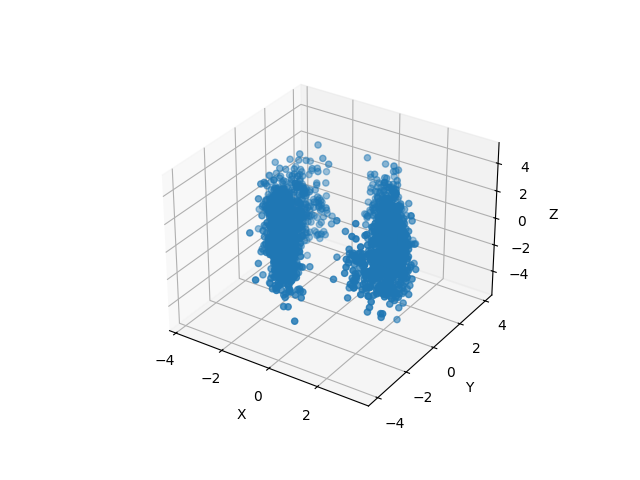
\includegraphics[width=0.55\textwidth]{latex_project/plots1/Clusters_informacion.png}
    \caption{Clusters de la información}
    \label{fig:clusters_originals}
\end{figure}

La figura \ref{fig:valores_singulares_X} muestra los valores singulares de la matriz $X$. Los valores singulares son el resultado de la descomposición en valores singulares (SVD), que descompone la matriz $X$ en tres matrices: $U$, $\Sigma$ y $V^T$. Estos valores singulares indican la cantidad de varianza que cada componente principal explica en los datos. Componentes con valores singulares más altos son más importantes porque explican más varianza en los datos originales.

\begin{figure}[H]
    \centering
    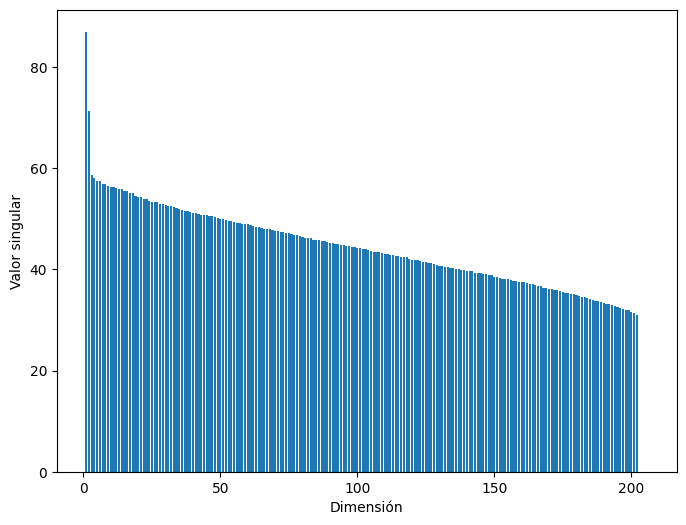
\includegraphics[width=0.65\textwidth]{latex_project/plots1/valores_singulares_martrizFULL.png}
    \caption{Valores singulares de $X$}
    \label{fig:valores_singulares_X}
\end{figure}

La figura \ref{fig:similarity_matrix} presenta las matrices de similitud para las distintas dimensiones. La matriz de similitud se calcula utilizando una función de similitud exponencial \ref{eq: Similitud} Esta visualización ayuda a entender cómo varía la similitud entre los puntos de datos a medida que se reduce la dimensionalidad. Cada matriz de similitud refleja la estructura interna de los datos en el espacio de dimensiones reducidas.

\begin{figure}[H]
    \centering
    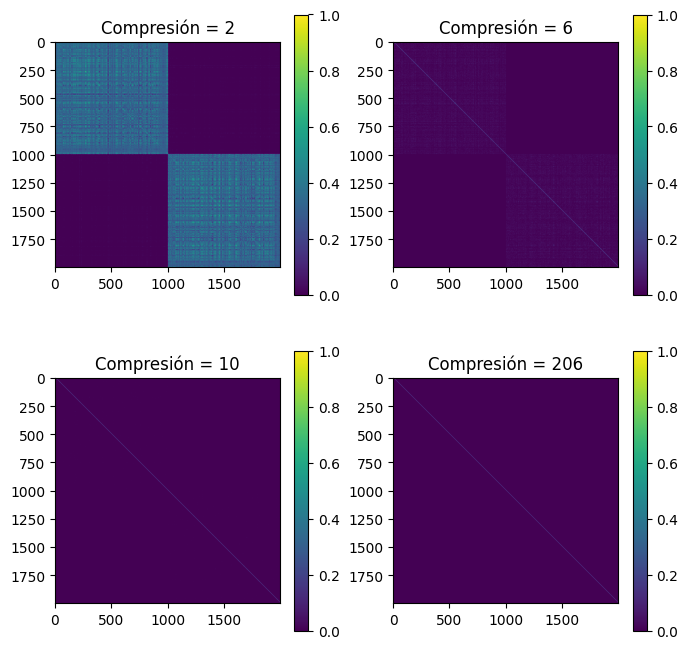
\includegraphics[width=0.65\textwidth]{latex_project/plots1/matriz_similaridad.png}
    \caption{Matrices de similitud para las distintas dimensiones}
    \label{fig:similarity_matrix}
\end{figure}
Luego, se calcularon las dimensiones mas importantes de la matriz. La importancia de cada dimensión reducida por $d$ se calcula como la suma de los cuadrados de los elementos en cada columna de \(V^T_d\):
   \[
   \text{Importancia}_j = \sum_{i=1}^d (V^T_d)_{ij}^2
   \]
   donde \((V^T_d)_{ij}\) es el elemento en la \(i\)-ésima fila y \(j\)-ésima columna de \(V^T_d\). De esta manera, se obtuvo que las dos dimensiones más importantes eran las dimensiones 205 y 203. A medida que se aumentaba la cantidad de dimensiones, se agregaban valores a esta lista manteniendo el orden. Para \(d=10\), las dimensiones más importantes son \(205, 203, 201, 202, 204, 200, 91, 28, 140, 69\). Estas dimensiones capturan la mayor parte de la variabilidad en los datos y son las más representativas en el espacio reducido de 10 dimensiones. Este conocimiento es útil para entender qué variables originales son más relevantes y pueden ser clave para la interpretación y análisis de los datos en estudios posteriores.


\subsubsection{Cuadrados Mínimos}


La figura \ref{fig:worst_best} muestra la aproximación de $X\beta$ a $Y$ utilizando modelos de regresión lineal con dimensiones 2 y 202. Aquí, $\beta$ es el vector de coeficientes del modelo de regresión. La aproximación se lleva a cabo proyectando los datos originales en un espacio de menor dimensión y luego ajustando el modelo de regresión lineal. El gráfico compara la precisión de las aproximaciones en dos escenarios: uno con una reducción drástica de dimensiones (2 dimensiones) y otro con casi todas las dimensiones originales (202 dimensiones). Estas dimensiones fueron elegidas ya que $d=2$ tiene un error alto mientras que $d=202$ es la dimensión donde la norma es mínima. 

\begin{figure}[H]
    \centering
    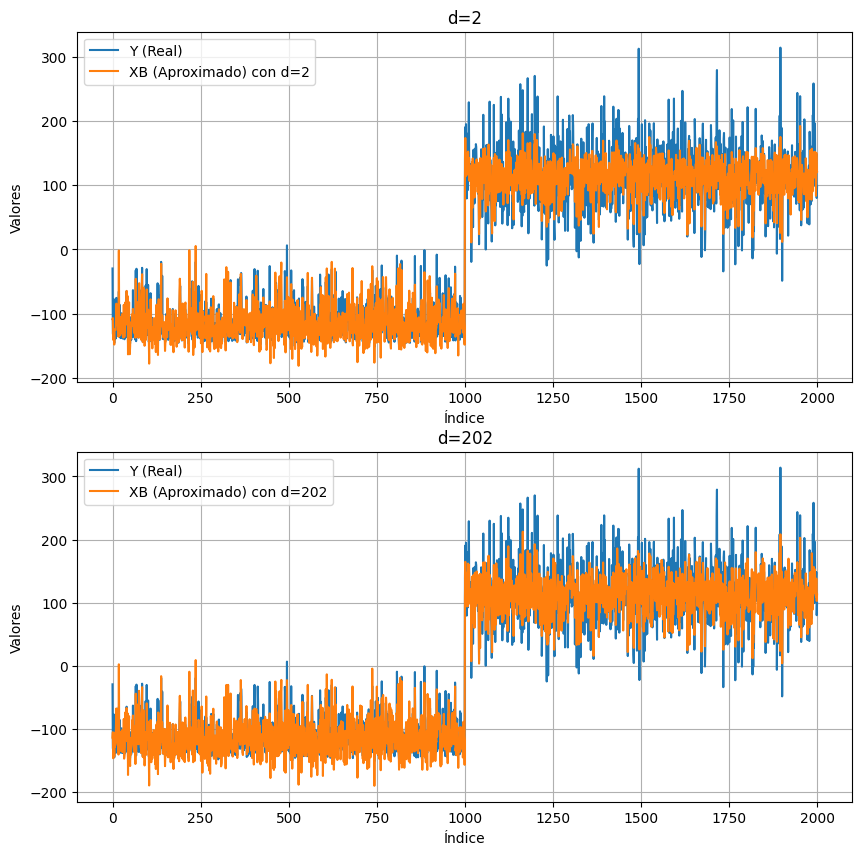
\includegraphics[width=0.65\textwidth]{latex_project/plots1/worst _best.png}
    \caption{Aproximación $X\beta$ de $Y$ con dimensión 2 y 202}
    \label{fig:worst_best}
\end{figure}

La figura \ref{fig:Norm_relative_error} presenta los errores relativos de la aproximación de $Y$ a medida que aumentan las dimensiones. El error relativo se calcula como la norma de la diferencia entre los valores predichos y los valores reales, normalizada por la norma de los valores reales. Este gráfico ilustra cómo el error de predicción disminuye a medida que se incrementa el número de dimensiones utilizadas en el modelo. La norma llega a un mínimo en la dimensión 202.

\begin{figure}[H]
    \centering
    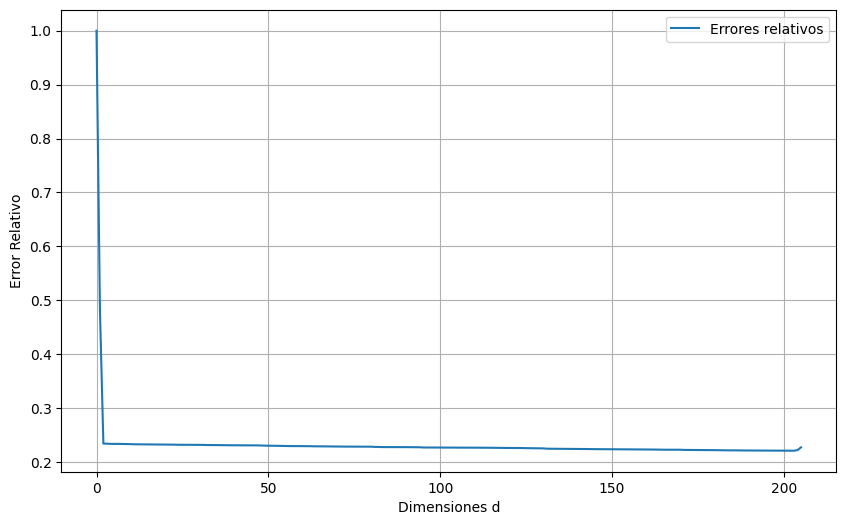
\includegraphics[width=0.65\textwidth]{latex_project/plots1/ERRORS_dimensiones.png}
    \caption{Errores relativos de la aproximación de $Y$ a medida que aumentan las dimensiones}
    \label{fig:Norm_relative_error}
\end{figure}






\subsection{Compresión de Imágenes}
Más adelante, se introdujo un archivo con 19 imágenes, que a su vez son matrices de $(p \times p)$, y se propuso comprimir la dimensión de estas imágenes a través de una descomposición en valores singulares (SVD).
\begin{figure}[H]
    \centering
    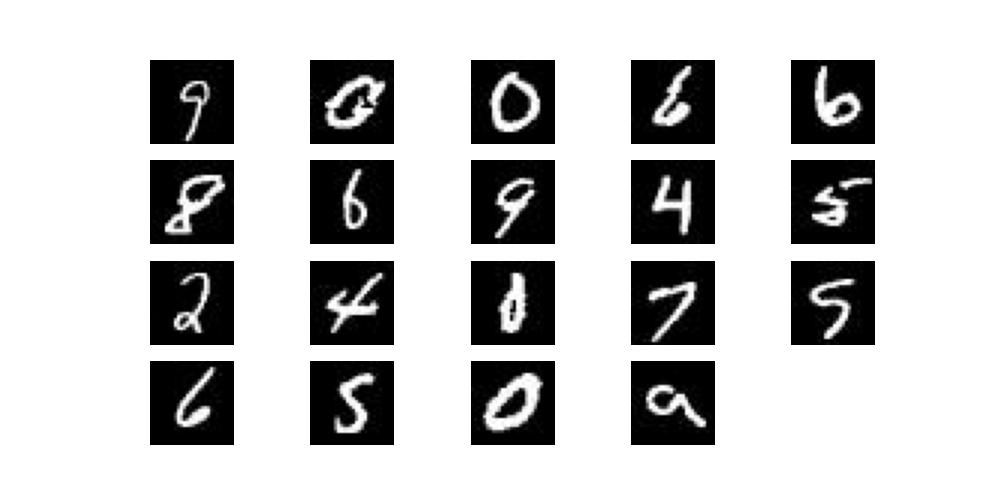
\includegraphics[width=0.65\textwidth]{latex_project/Graficos_ej2/original_images1.jpeg}
    \caption{Imágenes Originales, primer archivo}
    \label{fig:original_images1}
\end{figure}
\\

\subsubsection{Reconstrucciones de imágenes}
Para comenzar con la descomposición SVD, hay que tener en cuenta que cada imagen puede ser representada como un vector $x \in \mathbb{R}^{p*p}$. Sabiendo esto, se plasmaron todas las imágenes como vectores filas de una matriz de $\mathbb{R}^{n\text{x}(p*p)}$ y se realizó la descomposición SVD (\ref{SVD}) a esta matriz. Luego de la descomposición, se redujo la dimensionalidad de la matriz a dimensiones ($d$) 2, 6, 10 y 15. El proceso de reducción de dimensión consiste en, al multiplicar $U \Sigma V^{t}$, multiplicar únicamente las primeras $d$ columnas de la matriz $U$, los primeros $d$ valores singulares de la matriz diagonal $\Sigma$ y las primeras $d$ filas de la matriz $V^{t}$. Al hacer esto, se multiplican únicamente los componentes principales de la matriz original, es decir, los componentes donde se guarda mayor información sobre, en este caso, las imágenes. Esto se puede asegurar debido a que al descomponer en SVD, las tres matrices $U$, $\Sigma$ y $V^{t}$ cumplen que $u_1 \geq u_2 \geq ... \geq u_n$, $\sigma_1 \geq \sigma_2 \geq ... \geq \sigma_n$ y $v^{t}_1 \geq v^{t}_2 \geq ... \geq v^{t}_n$ respecto de la importancia en la carga de información. Esta cualidad se puede observar en los gráficos a continuación.

\begin{figure}[H]
    \centering
    \begin{subfigure}{0.45\textwidth}
        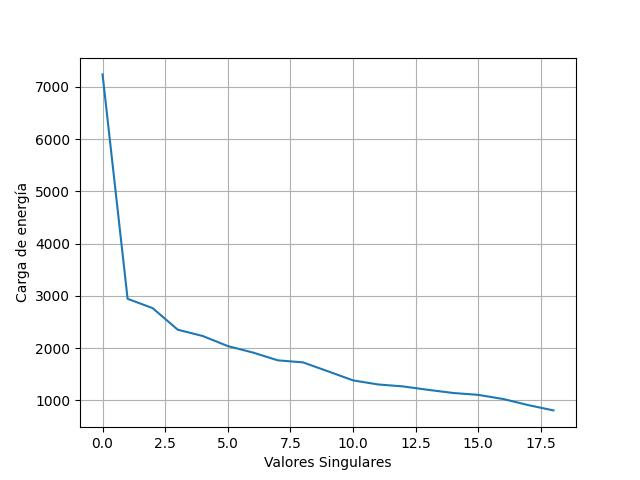
\includegraphics[width=\linewidth]{latex_project/Graficos_ej2/singular_values.jpeg}
        \caption{Carga de Energía de los Valores Singulares}
        \label{fig:singular_values}
    \end{subfigure}
    \hfill
    \begin{subfigure}{0.45\textwidth}
        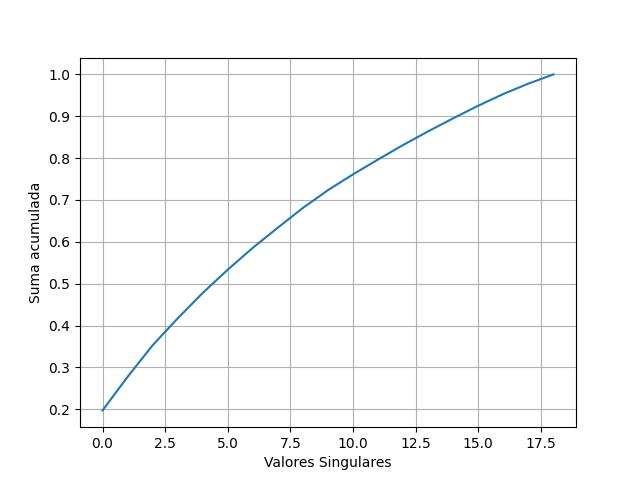
\includegraphics[width=\linewidth]{latex_project/Graficos_ej2/cumulative_sum.jpeg}
        \caption{Suma Acumulada de los Valores Singulares}
        \label{fig:sv_cumsum}
    \end{subfigure}
    \caption{Gráficos de Valores Singulares}
    \label{fig:sv_graphs}
\end{figure}

En la figura \ref{fig:singular_values} queda clara la realción entre los valores singulares y su carga de energía. Se puede ver que en los primeros valores singulares la carga de energía es muy alta y además se ve una caída drástica hasta cierto valor con una estabilización posterior. Rotunda o controlada, se ve que la caída en la carga de energía a medida que aumentan los valores singulares es constante, represetando el ordenamiento de los mismos en cuanto a su importancia.
\\

Seguido del análisis de los valores singulares, se visualizaron las imágenes reconstruidas a las dimensiones ($d$) mencionadas anteriormente

\begin{figure}[H]
    \centering
    \begin{subfigure}{0.45\textwidth}
        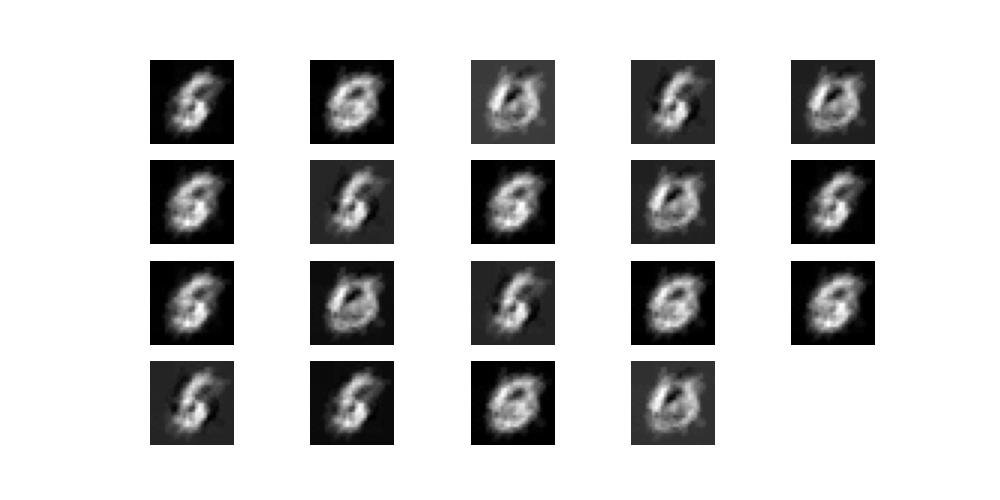
\includegraphics[width=\linewidth]{latex_project/Graficos_ej2/compression_2.jpeg}
        \caption{Compresión $d = 2$}
        \label{fig:d2}
    \end{subfigure}
    \hfill
    \begin{subfigure}{0.45\textwidth}
        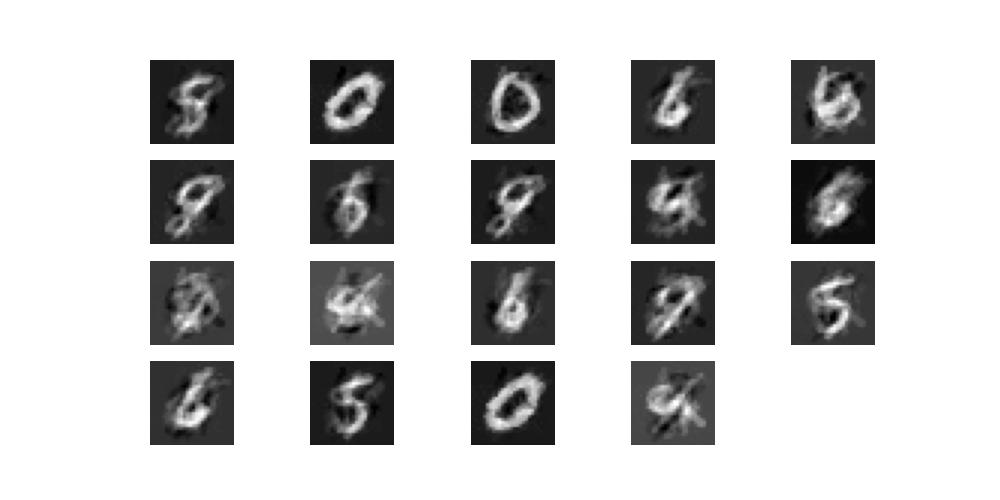
\includegraphics[width=\linewidth]{latex_project/Graficos_ej2/compression_6.jpeg}
        \caption{Compresión $d = 6$}
        \label{fig:d6}
    \end{subfigure}
    \\
    \begin{subfigure}{0.45\textwidth}
        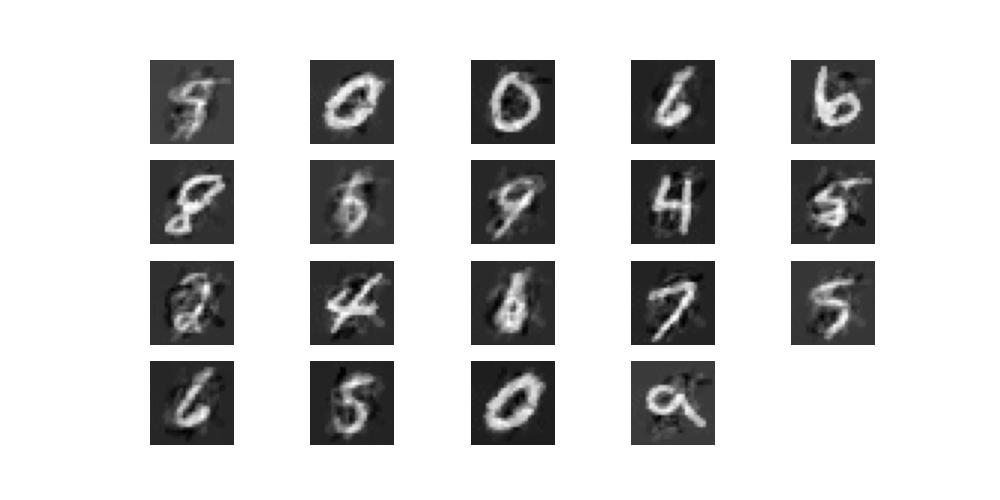
\includegraphics[width=\linewidth]{latex_project/Graficos_ej2/compression_10.jpeg}
        \caption{Compresión $d = 10$}
        \label{fig:d10}
    \end{subfigure}
    \hfill
    \begin{subfigure}{0.45\textwidth}
        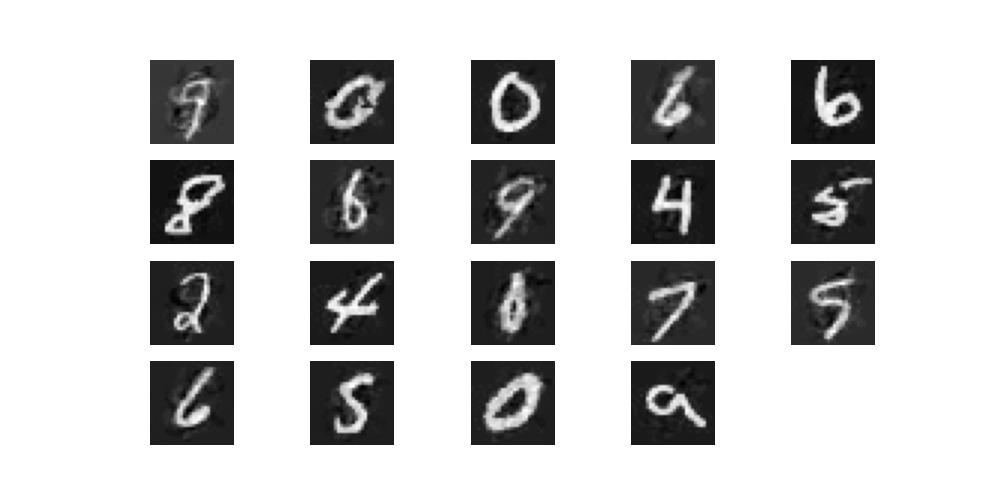
\includegraphics[width=\linewidth]{latex_project/Graficos_ej2/compression_15.jpeg}
        \caption{Compresión $d = 15$}
        \label{fig:d15}
    \end{subfigure}
    \caption{Compresión de imágenes en diferentes dimensiones ($d$)}
    \label{fig:compresiones}
\end{figure}

Analizando las 4 reconstrucciones, se ve que al hacerlo en dos dimensiones no se distinguen mucho las imágenes, ya que, por más que sean los vectores y valores singulares con mayor información sobre las matrices, la dimensión es baja como para representar las imágenes de manera precisa. En cambio, al subir la dimensión a 6, las imágenes se comienzan a distinguir mejor. Innegablemente no se ven reconstrucciones perfectas, pero la mayoría de las 19 representaciones se diferencian una de otra. Ya subiendo la dimensionalidad de las reconstrucciones a 10 y luego a 15 las imágenes son cada vez más parecidas a las originales, demostrando que estas últimas dimensiones agregan detalles a las mismas. Queda claro que los primeros vectores y valores singulares son los que esbozan los factores principales de las matrices, mientras que los vectores y valores singulares finales son de alguna manera despreciables para el análisis.
\\

\subsubsection{Similaridad de Imágenes}
La similaridad a la que se hace referencia puede ser graficada al comparar cada fila consigo misma y todas las otras filas de la matriz que contiene como vectores fila las imágenes reducidas representadas en vectores $x_i \in \mathbb{R}^{(p*p)}$ con el uso de la función de similaridad del coseno (matriz de coseno) \cite{wikipedia_cosine_similarity}. Se produjo la matriz de similaridad para cada una de las reducciones realizadas anteriormente a las dimensiones ($d$) 2, 6, 10 y 15.

\begin{figure}[H]
    \centering
    \begin{subfigure}{0.45\textwidth}
        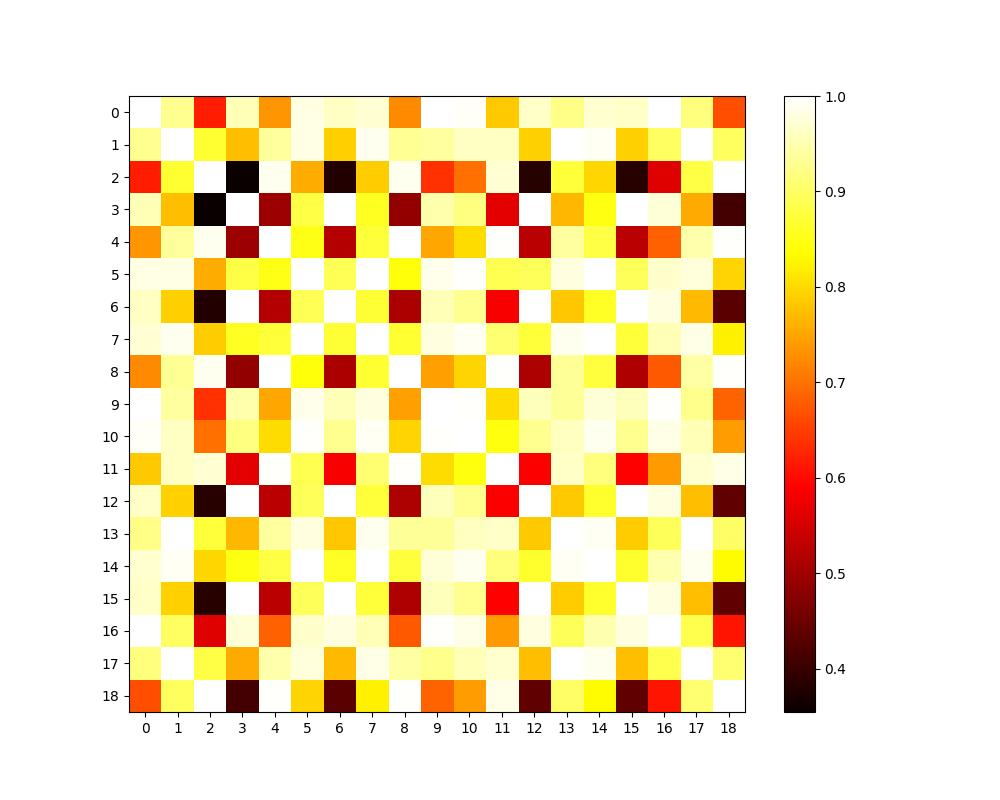
\includegraphics[width=\linewidth]{latex_project/Graficos_ej2/similarity_matrix_2.jpeg}
        \caption{Matriz de similaridad para $d = 2$}
        \label{fig:similarity_d2}
    \end{subfigure}
    \hfill
    \begin{subfigure}{0.45\textwidth}
        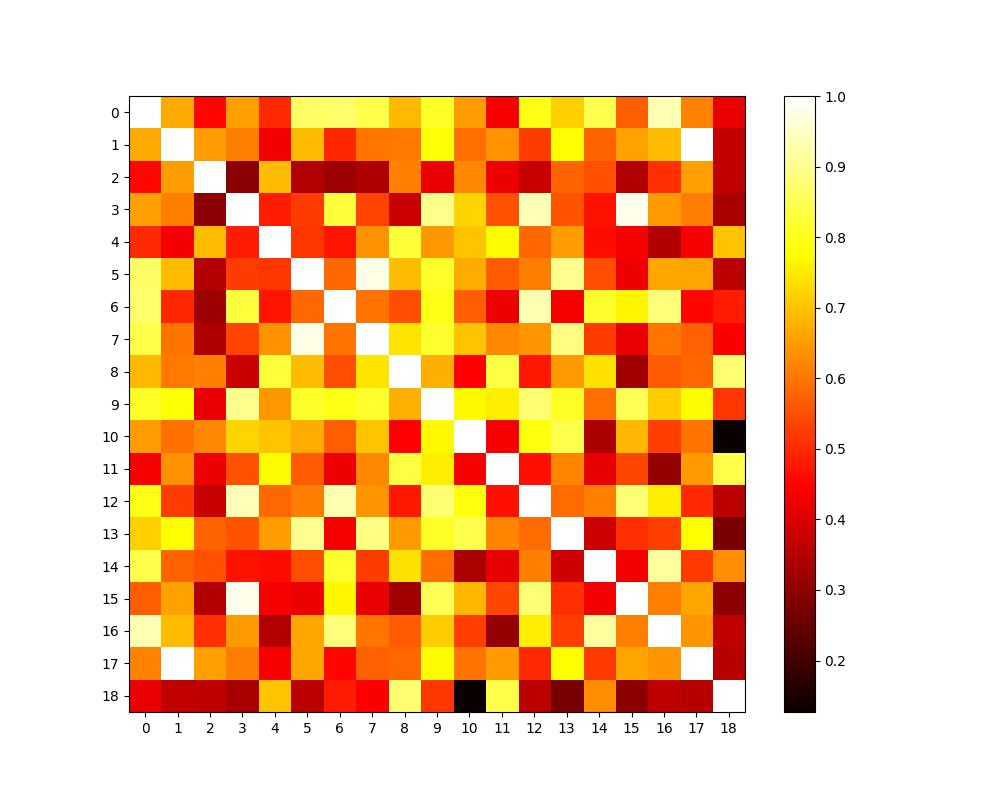
\includegraphics[width=\linewidth]{latex_project/Graficos_ej2/similarity_matrix_6.jpeg}
        \caption{Matriz de similaridad para $d = 6$}
        \label{fig:similarity_d6}
    \end{subfigure}
    \\
    \begin{subfigure}{0.45\textwidth}
        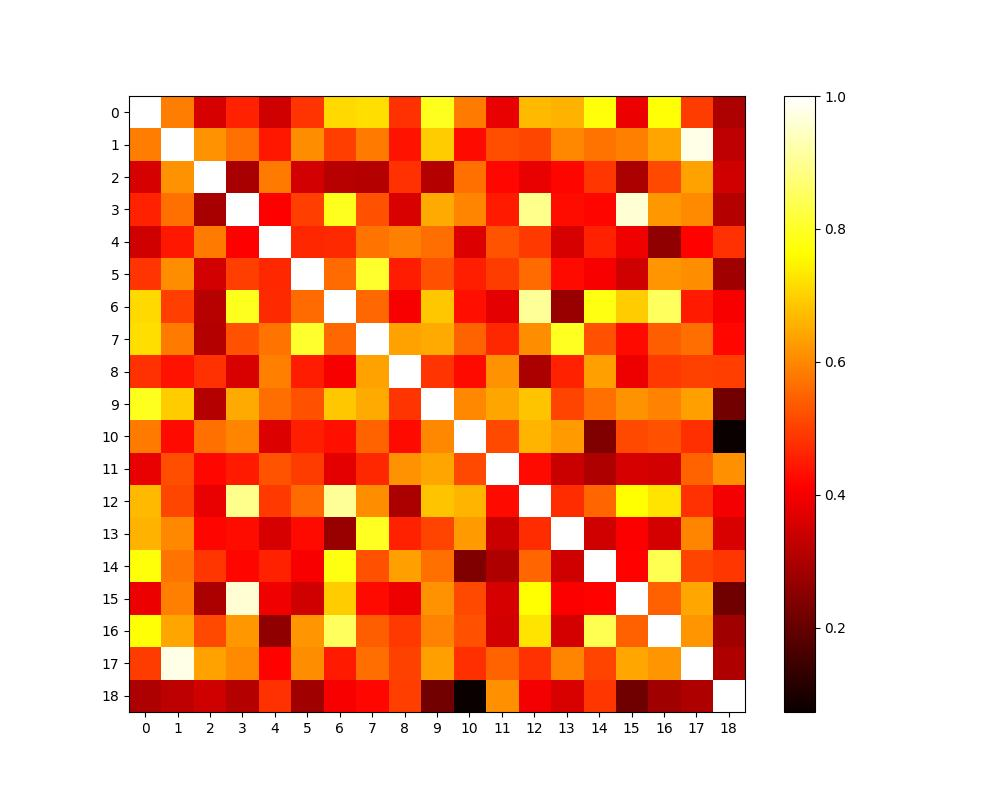
\includegraphics[width=\linewidth]{latex_project/Graficos_ej2/similarity_matrix_10.jpeg}
        \caption{Matriz de similaridad para $d = 10$}
        \label{fig:similarity_d10}
    \end{subfigure}
    \hfill
    \begin{subfigure}{0.45\textwidth}
        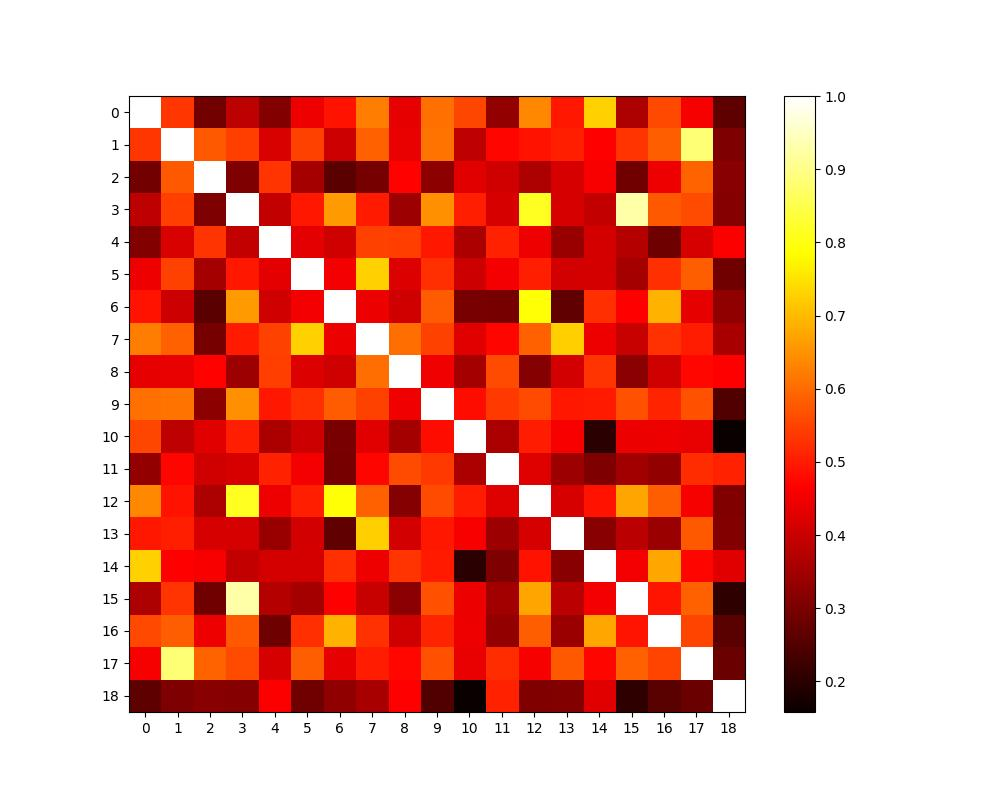
\includegraphics[width=\linewidth]{latex_project/Graficos_ej2/similarity_matrix_15.jpeg}
        \caption{Matriz de similaridad para $d = 15$}
        \label{fig:similarity_d15}
    \end{subfigure}
    \caption{Matrices de similaridad para diferentes dimensiones ($d$)}
    \label{fig:similarity_matrices}
\end{figure}

Antes de analizar cada matriz hay que entender qué representan los colores de las mismas. En las matrices presentadas arriba, los mayores valores representan una mayor similaridad vector a vector (imagen a imagen). Cuanto más claro sea el color del punto $A_{i,j}$, más similaridad hay entre las dos imágenes siendo comparadas. Lógicamente, la diagonal de todas las matrices contiene únicamente componenetes totalmente blancos, ya que la diagonal representa la comparación de cada iamgen con sí misma. Luego, se da una tendencia que a más dimensiones utilizadas para la reconstrucción, la mayoría de los puntos $A_{i,j}$ se tornan más rojos, es decir que hay menos similaridad hay entre las imágenes. Sabiendo esto, se hacen visible las imágenes que son más similares entre sí y las que no. Analizando más que nada las matrices con mayor dimensión en la reconstrucción, se ve una alta similaridad en la comparación de las imágenes 3 y 15, manteniendo un color claro para todos los diferentes valores de $d$. Por el otro lado, es visible la poca similaridad en la comparación de las imágenes 10 y 18. Aunque en dimensión $d = 2$ no son las imágenes menos similares entre sí, en el resto de las dimensiones, el componente $A_{i,j}$ es muy oscuro, mostrando altas diferencias entre estas imágenes. Comparando las matrices de similaridad con las imágenes reconstruidas, esto cobra mucho sentido dado que en una dimensión menor, las imágenes son menos claras y se parecen entre sí. A medida que las dimensiones aumentan, las reconstrucciones son cada vez más claras, con más detalle, por lo que se parecen menos entre sí.
\\

\subsubsection{Cambio de Base}
Finalmente, se presentó un segundo archivo con otras 8 imágenes, matrices de $(p \times p)$, y se pidió calcular la dimensión mínima para la cual es posible comprimir las imágenes tal que el error entre las imágenes originales y las reconstrucciones sea menor al 10\% bajo la norma de Frobenius \ref{Frobenius}.

\begin{figure}[H]
    \centering
    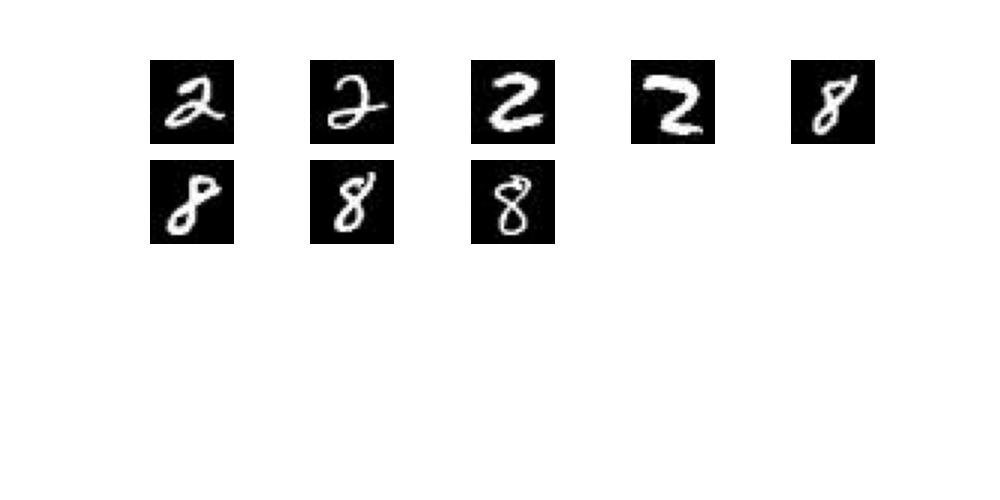
\includegraphics[width=0.65\textwidth]{latex_project/Graficos_ej2/original_images2.jpeg}
    \caption{Imágenes Originales, segundo archivo}
    \label{fig:original_images2}
\end{figure}

En primer lugar se realizó la misma descomposición SVD (\ref{SVD}) que para el primer archivo de imágenes, pero en este caso se iteró reduciendo la dimensionalidad de la matriz una dimensión a la vez mientras se calculaba el error realtivo bajo la norma de Frobenius. La idea de este procedimiento era llegar a la conclusión de que la primera dimensión cuya reducción cumpla con un error menor al 10\% sería la dimensión óptima que se buscaba. Sin embargo, luego de las iteraciones necesarias, todas las dimensiones menores a 8, que sería la dimensionalidad completa presentaban un error mayor al 10\%. Fue por esta razón que se concretó que la dimensión óptima era $d = 8$.

\begin{figure}[H]
    \centering
    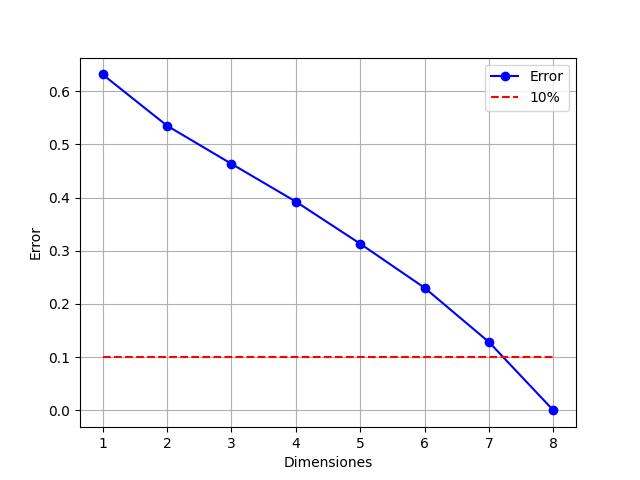
\includegraphics[width=0.65\textwidth]{latex_project/Graficos_ej2/error.jpeg}
    \caption{Error Relativo de Reconstrucción bajo la norma de Frobenius}
    \label{fig:error}
\end{figure}

Una vez calculada la dimensión óptima ($d = 8$) se planteó el problema de reconstruir las imágenes del primer archivo presentado bajo la base de la descomposición de la segunda matriz de imágenes. Para esto, es necesario utilizar los autovectores de la base de reconstrucción de la segunda descompsición. En una descomposición SVD, los autovectores mencionados se encuentran almacenados en la matriz $V^{t}$. Por ende, la manera de reconstruir las imágenes del primer archivo con la base de autovectores de la segunda descomposición es multiplicando la matriz reconstruida $d = 8$ del primer problema por la matriz $V^{t}$ otra vez transpuesta, es decir $(V^{t})^{t}$, o simplemente $V$, y nuevamente por $V^{t}$.

$Matriz$ $con$ $Base$ $Cambiada$ $(A_{d8}$ $reconstruida$ $con$ $la$ $base$ $de$ $la$ $segunda$ $descomposición):$
\begin{equation}
    \centering
    \begin{bmatrix}
            &   &   \\
            &CB &   \\
            &   &   
    \end{bmatrix} = \begin{bmatrix}
            &   &   \\
            &A_{d8}&    \\
            &   &   
    \end{bmatrix}\begin{bmatrix}
            &   &   \\
            & V &   \\
            &   &   
    \end{bmatrix}\begin{bmatrix}
            &   &   \\
            &V^{t}& \\
            &   &
    \end{bmatrix}
\end{equation}

Luego de realizar la multiplicación de matrices previa en el caso pertinente, se llega a la siguiente representación de las imágenes del primer archivo reducidas a dimensión $d = 8$.

\begin{figure}[H]
    \centering
    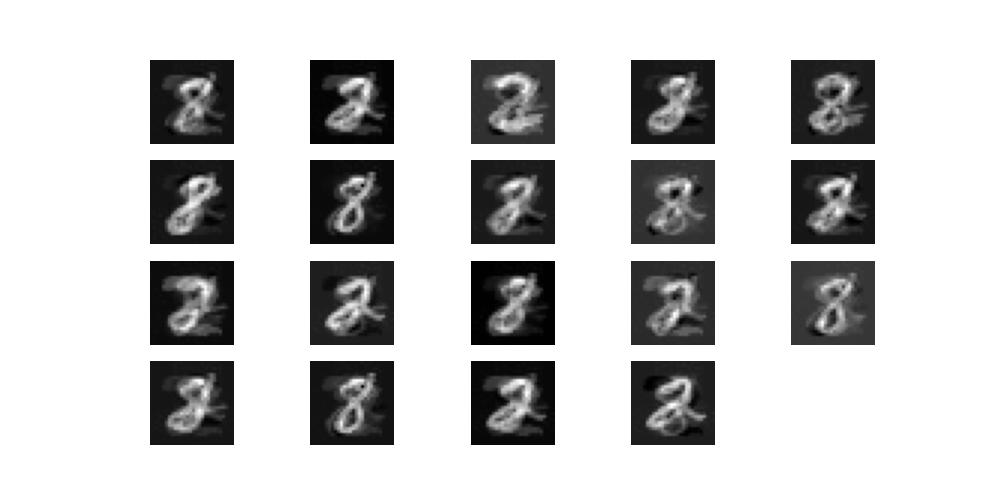
\includegraphics[width=0.65\textwidth]{latex_project/Graficos_ej2/compression_8.jpeg}
    \caption{Reconstrucción de imágenes del primer archivo en $d = 8$ utilizando la base de vectores singulares la segunda descomposición}
    \label{fig:d8}
\end{figure}

Es evidente que la reconstrucción de las imágenes no es la mejor en esta dimensión. Igualmente esto sigue una cierta lógica. Si se vuelve a mirar las imágenes originales del segundo archivo en la figura \ref{fig:original_images2}, vemos que estas son todas ochos y dos diferentes. Teniendo en cuenta esto, la base de la descomposición guarda gran información de estos ochos y dos en sus autovectores, los cuales luego se utilizan para la última reducción de dimensionalidad. Esto quiere decir que se están queriendo representar otros números con la base de ochos y dos de la segunda descomposición. El error relativo de reconstrucción se puede calcular analíticamente además de ser notorio a simple vista. Para lograrlo, se le aplicó la norma de Frobenius a la resta entre la matriz de imágenes del primer archivo reconstruida a $d = 8$ y la matriz reconstruida con la base cambiada.

\begin{equation}
    \centering
    \left|\left|\begin{bmatrix}
            &   &   \\
            &CB &   \\
            &   &   
    \end{bmatrix} - \begin{bmatrix}
            &   &   \\
            &A_{d8}&    \\
            &   &   
    \end{bmatrix}\right|\right|_F \approx 0,7502 = 75,02\%
\end{equation}

Al hacer el cálculo del error relativo se descartan dudas sobre el tamaño del error en la reconstrucción realizada.

\section{Conclusión}
En lo que respecta a la compresión de imágenes a través de descomposiciones SVD y truncamiento del producto, luego de un detallado análisis se llega a la conclusión de que no son neceesarias todas las dimensiones de una matriz para dar una reconstrucción fehaciente de la imagen que esta representa. El primer vector y valor singular almacenados en orden en las respectivas matrices de la descomposición guardan mayor información que el siguiente, y así sucesivamente, por lo que únicamente es necesario hacer uso de un número $d$ tal que $d \leq r,$ con $r$ rango de la matriz, de dimensiones para construir una imagen similar.
\\

Además, se entendió que la base de vectores singulares es importante a la hora de la reconstrucción de una matriz en una dimensionalidad menor dado que una base muy específica puede no ayudar para la reconstrucción de otros modelos que no sean el modelo que la misma base representa.

\appendix




\printbibliography



\end{document}